\section*{Въпроси}

\begin{questions}

  \question[6] Какви са предимствата на използването на разслоени архитектури в
  компютърните мрежи? (Изберете три отговора)

  \begin{choices}
    \choice Горните слоеве могат да предоставят услуги на слоевете под тях.

    \CorrectChoice Сложната задача за провеждане на комуникация се разпада на
    по-малки задачи.

    \CorrectChoice Имплементациите на долните слоеве могат да бъдат променяни, без
    да бъдат променяни имплементациите на тези над тях, защото интерфейсите им не
    се променят.

    \CorrectChoice По-ниските слоеве скриват имплементационни детайли от
    по-високите.
  \end{choices}

  \question[6] Ако вземем в предвид \foreignlanguage{english}{DoD (TCP/IP)}
  модела, как протоколните единици данни (\foreignlanguage{english}{protocol
    data units} или \foreignlanguage{english}{PDUs}) на един слой се
  енкапсулират от по-нисък слой? (Изберете два верни отговора)

  \begin{choices}
    \choice В изходяща посока, новата протоколна единица от данни бива
    конструирани от комбинация от данни от слоевете под и над енкапсулиращия слой.

    \CorrectChoice Протоколната единица данни на даден слой е съставена от поле от
    данни, състоящо се единствено от цялата протоколна единица данни на горния
    слой, и заглавна част (\foreignlanguage{english}{header}), описваща тези
    данни.

    \choice В Интернет, всички данни, които пристигат от мрежовия слой, трябва да
    преминат през TCP слоя, преди да достигнат приложението.

    \CorrectChoice Във входяща посока, частта от протоколната единица данни, която
    съставлява данните, се предава на горния слой.
  \end{choices}

  \question[6] Кои от следните твърдения са верни? (Изберете два отговора)
  \begin{choices}
    \CorrectChoice Последствие от използването на разслоени модели в компютърните
    мрежи, е това, че даден слой при източника на данните комуникира със същия
    слой при приемника на данните, без оглед на имплементационните детайли на
    слоевете под и над него.

    \choice 7-слойният OSI модел е по-добър от 4-слойния
    \foreignlanguage{english}{DoD} (TCP) модел, защото позволява на мрежите да
    бъдат по-надеждни.

    \CorrectChoice Приложно-програмният интерфейс (API) на сокетите предоставя на
    компютърните приложения преизползваеми средства за комуникация с отдалечени
    приложения.

    \choice Мрежовият слой разчита на състоянието на връзката, поддържано от
    транспортния слой, за да следи с кого комуникира.
  \end{choices}\question[6] Какво \emph{НЕ} се случва, когато рамка
  (\foreignlanguage{english}{frame}) бъде получена от комутатор
  (\foreignlanguage{english}{switch}) на втори слой? (Изберете три отговора)

  \begin{choices}
    \choice Комутаторът ще направи решение за пренасочване
    (\foreignlanguage{english}{forwarding decision}) на базата на адресът на
    получател от \foreignlanguage{english}{Ethernet} хедъра.

    \CorrectChoice Комутаторът ще енкапсулира рамката отново с нов Ethernet хедър,
    в който адресът на източникът ще бъде MAC адресът на комутатора.

    \CorrectChoice Комутаторът ще трябва да научи IP адреса на получателя, за да
    направи избор за пренасочване.

    \CorrectChoice За да провери коректността на данните, комутаторът ще трябва
    да извлече данните на приложението от рамката.
  \end{choices}

  \question[6] Кои от следните твърдения са верни за IP? (Изберете три отговора)
  \begin{choices}
    \CorrectChoice Интернет протоколът (IP) е пример за протокол от мрежовия
    слой на OSI модела.

    \CorrectChoice В момента за комуникация в Интернет се използват основно две
    версии на IP – IP версия 4 и IP версия 6.

    \choice IP е пример за протокол от транспортния слой на OSI модела и
    предоставя надеждна комуникация.

    \CorrectChoice IP не гарантира, че пакетите ще бъдат доставени в реда, в
    който са изпратени или изобщо.
  \end{choices}

  \question[6] Кое от следните твърдения е вярно за IP?
  \begin{choices}
    \choice IP датаграмите (\foreignlanguage{english}{datagram}) съдържат поле
    "`\texttt{\foreignlanguage{english}{hop-count}}"', към чиято стойност бива
    добавена единица всеки път, когато датаграмата премине през маршрутизатор
    (\foreignlanguage{english}{router}).

    \choice IP датаграмите съдържат
    \texttt{\foreignlanguage{english}{time-to-live}} поле, което се състои от
    списък на всички маршрутизатори, през които е преминал пакетът, за да може
    крайният хост да установи дали пакета е бил затворен в цикъл.

    \CorrectChoice IP датаграмите съдържат целочислено поле, на базата на чиято
    стойност се открива и прекратява препредаването им в безкраен цикъл.

    \choice \texttt{\foreignlanguage{english}{time-to-live}} полето пренася
    данни от транспортния слой.
  \end{choices}

  \question[6] Кои от следните твърдения не са верни за IP? (Изберете три
  отговора)
  \begin{choices}
    \CorrectChoice \texttt{\foreignlanguage{english}{time-to-live}} полето
    пренася данни от транспортния слой.

    \choice IP датаграмите съдържат целочислено поле, на базата на чиято
    стойност се открива и прекратява препредаването им в безкраен цикъл.

    \CorrectChoice IP датаграмите съдържат
    \texttt{\foreignlanguage{english}{time-to-live}} поле, което се състои от
    списък на всички маршрутизатори, през които е преминал пакетът, за да може
    крайният хост да установи дали пакета е бил затворен в цикъл.

    \CorrectChoice IP датаграмите (\foreignlanguage{english}{datagram}) съдържат
    поле "`\texttt{\foreignlanguage{english}{hop-count}}"', към чиято стойност
    бива добавена единица всеки път, когато датаграмата премине през
    маршрутизатор (\foreignlanguage{english}{router}).
  \end{choices}

  \question[6] Маршрутизаторът (\foreignlanguage{english}{router}) може да
  отхвърля пакети, когато няма налични ресурси за обработката им. Има обаче
  случаи, когато ресурси за обработката на пакетите са налични, но въпреки това
  маршрутизаторът ги отхвърля. Кои от следните са примери за сценарии, в които
  маршрутизатор отказва да обработи пакети, въпреки че има наличните за това
  ресурси? (Изберете две)

  \begin{choices}
    \choice При претоварена с данни връзка.

    \CorrectChoice Маршрутизаторът е конфигуриран като
    \foreignlanguage{english}{firewall} и това диктува кои пакети трябва да
    бъдат отхвърлени и кои -- обработени.

    \CorrectChoice Доставчик на Интернет ограничава широчината на лентата
    (\foreignlanguage{english}{bandwidth}), която потребителите могат да
    използват, въпреки че има достатъчен капацитет.

    \choice При пристигане на пакет, чиято контролна сума
    (\foreignlanguage{english}{checksum}) показва, че в него има грешка.
  \end{choices}

  \question[6] Кои от следните твърдения са верни относно
  \foreignlanguage{english}{TCP}? (Изберете два отговора)
  \begin{choices}
    \choice \foreignlanguage{english}{TCP} използва контролна сума, за да
    установи дали данните на приложенията се придържат към правилния синтаксис.

    \choice Тъй като \foreignlanguage{english}{TCP} кодира данните с код, който
    коригира грешки, никога не се налага да се изпращат наново липсващи
    сегменти.

    \CorrectChoice \foreignlanguage{english}{TCP} доставя надеждно и в
    правилната подредба поток от байтове от единия до другия участник в
    комуникацията.

    \CorrectChoice Когато \foreignlanguage{english}{TCP} пакет достигне до
    дестинацията си, данните, които той пренася, биват доставени до услугата или
    приложението, посочени от порта на дестинацията
    (\foreignlanguage{english}{destination port}).

    \choice Тъй като \foreignlanguage{english}{TCP} не може да разчита на
    IP да форматира пакетите правилно, IP адресът на дестинацията трябва да бъде
    включен в TCP хедъра.
  \end{choices}

  \question[6] TCP е отговорен за предоставянето на надеждно, последователно
  доставяне на данни между приложения. Кои от следните са директни последствия
  от изборите, направени при проектирането на TCP? (Изберете два отговора)
  \begin{choices}
    \choice TCP е самодостатъчен и наличната адресна информация в TCP хедъра
    позволява при провеждане на комуникация да не се използва мрежовия слой или
    който и да е друг по-нисък слой.

    \choice TCP не изисква състоянието на връзката да бъде установено преди
    участниците в комуникацията да започнат да обменят данни.

    \CorrectChoice TCP ще изпрати отново липсващите данни, дори ако приложението
    не може да ги използва -- например при Интернет телефонията -- закъснели
    данни може да пристигнат прекалено късно, за да бъдат полезни.

    \CorrectChoice TCP спестява нуждата в приложението да бъдат имплементирани
    механизми за преизпращане на неполучени данни или преподреждане на данни,
    получени в неправилен ред данни.

    \choice TCP може да функционира, само ако слоят под него също гарантира
    надеждност и последователност на данните.
  \end{choices}

  \question[6] Преди да започне комуникацията, TCP установява нова връзка
  посредством тристранно ръкостискане (\foreignlanguage{english}{three-way
    handshake}). Това е така, защото:
  \begin{choices}

    \CorrectChoice При TCP, крайните точки пазят информация за състоянието на
    комуникацията в двете посоки и ръкостискането позволява това състояние да
    бъде инициализирано и синхронизирано.

    \choice Традицията налага, когато двама души се запознаят, да си стиснат
    ръцете.

    \choice Вместо тристранно, TCP може да използва двустранно
    ръкостискане. Третата стъпка е въведена единствено, за да се предотврати
    подслушването на данните.

    \CorrectChoice TCP установява поток от данни и в двете посоки. Тристранното
    ръкостискане позволява двата потока от данни да бъдат установени и потвърдени.
  \end{choices}

  \question[6] Сравнен с TCP, UDP е много по-прост протокол. Той е безвръзков и
  не предоставя надеждно предаване на данните. Кои от следните твърдения,
  относно UDP, са верни?
  \begin{choices}
    \choice Никое приложение не би искало да използва UDP, защото не предоставя
    надежден транспорт на данните.

    \CorrectChoice UDP често се използва за разпръскване
    \foreignlanguage{english}{broadcast} на данни, защото не изисква
    установяването на състояние за всеки получател на данните.

    \CorrectChoice За кратка комуникация от вид "`заявка-отговор"', използвана
    например при DNS, се предпочита използването на UDP, за да се избегнат
    служебните разходи (\foreignlanguage{english}{overhead}) на TCP.

    \CorrectChoice UDP е подходящ за приложения, които не се нуждаят
    задължително от надежден транспорт на данни
    (пр. \foreignlanguage{english}{voice-over-IP}, онлайн игри).
  \end{choices}

  \question[6] Комутационните мрежи (\foreignlanguage{english}{packet-switched
    networks}) не позволяват няколко източници и дестинации на пакети да споделят
  една и съща връзка.
  \begin{oneparchoices}
    \choice Вярно.
    \CorrectChoice Грешно.
  \end{oneparchoices}

  \question[6] Всички пакети, които имат еднакви източник и дестинация трябва да
  преминат през едно и също множество от връзки и комутатори.
  \begin{oneparchoices}
    \choice Вярно.
    \CorrectChoice Грешно.
  \end{oneparchoices}

  \question[6] Кое от изброените е полезен товар
  (\foreignlanguage{english}{payload}) в протоколната единица данни на протокол
  от каналния слой на OSI модела?
  \begin{oneparchoices}
    \choice IP пакет

    \CorrectChoice Ethernet сегмент

    \choice Потребителски данни

    \choice TCP рамка
  \end{oneparchoices}

  \question[6] Кои от следните са следствия от енкапсулацията на данните?
  \begin{choices}
    \CorrectChoice Запазване на разделението на слоевете на архитектурата.

    \choice Изпращане на по-голямо количество данни по мрежата.

    \CorrectChoice Опростяване на имплементацията на слоевете на архитектурата.

    \choice Защита от злонамерени атаки.
  \end{choices}

  \question[6] TCP сегмент може да енкапсулира полезен товар
  (\foreignlanguage{english}{payload}), в който има друг TCP сегмент.
  \begin{oneparchoices}
    \CorrectChoice Вярно.

    \choice Грешно.
  \end{oneparchoices}

  \question[6] Кой слой се намира между физическия и мрежовия слой?
  \begin{oneparchoices}
    \choice Сесийният.

    \choice Транспортният.

    \CorrectChoice Каналният.

    \choice Презентационният.
  \end{oneparchoices}

  \question[6] Изберете правилното продължение на изречението "`Разслояването
  (\foreignlanguage{english}{layering})..."'
  \begin{choices}
    \choice пречи на злонамерени актьори да компрометират кода.

    \choice позволява на инженерите да се справят със сложността като
    разделят проблема на части с добре дефинирани интерфейси помежду им.

    \choice твърди, че някои операции трябва да бъдат изпълнени на различни
    хостове в мрежата.
  \end{choices}

  \question[6] Всеки маршрутизатор (\foreignlanguage{english}{router}) може да
  бъде свързан най-много с два други маршрутизатора.
  \begin{oneparchoices}
    \choice Вярно.
    \CorrectChoice Грешно.
  \end{oneparchoices}

  \question[6] Целта на маршрута по премълчаване
  (\foreignlanguage{english}{default route}) е да покаже накъде трябва да бъдат
  пренасочени пакетите, чиято дестинация не съвпада с никой друг запис в
  маршрутната таблица.
  \begin{oneparchoices}
    \CorrectChoice Вярно.
    \choice Грешно.
  \end{oneparchoices}

  \question[6] Сегменти с вдигнат \texttt{FIN} флаг се изпращат при създаване на
  TCP връзка.
  \begin{oneparchoices}
    \choice Вярно.
    \CorrectChoice Грешно.
  \end{oneparchoices}

  \question[6] Кои от следните адреси са част от мрежата \texttt{192.13.128.0} с
  мрежова маска \texttt{255.255.128.0}?
  \begin{choices}
    \CorrectChoice 192.13.128.0
    \CorrectChoice 192.13.255.1
    \CorrectChoice 192.13.255.64
    \choice 192.13.0.0
    \choice 192.13.64.2
    \CorrectChoice 192.13.192.255
  \end{choices}

  \question[6] Вярно ли е, че мрежа с представка "`\texttt{/8}"' съдържа
  $2^{24}$ адреса, които могат да бъдат зачислени на хостове?
  \begin{oneparchoices}
    \choice Вярно.
    \CorrectChoice Грешно.
  \end{oneparchoices}


  \question[6] Вярно ли е, че мрежа с представка "`\texttt{/8}"' съдържа
  $2^8$ адреса, които могат да бъдат зачислени на хостове?
  \begin{oneparchoices}
    \choice Вярно.
    \CorrectChoice Грешно.
  \end{oneparchoices}

  \question[6] Вярно ли е, че подмрежа с маска \texttt{255.255.64.0} съдържа
  повече адреси от такава с маска \texttt{255.255.8.0}?

  \begin{oneparchoices}
    \choice Вярно.
    \CorrectChoice Грешно.
  \end{oneparchoices}

  \question[6] Посочете вярното твърдение, относно NAT.
  \begin{choices}
    \choice Невъзможно е хостовете, намиращи се зад NAT да инициират връзки с Интернет.
    \choice Замисълът на NAT е да прочита всички пакети и да пропуска само безопасните.
    \CorrectChoice Възможно е да се използва верига от повече от един
    маршрутизатор, извършващ NAT.
  \end{choices}

  \question[6] Външен хост се опитва да създаде TCP връзка с хост, слушащ на
  порт \texttt{5577} зад NAT (\foreignlanguage{english}{Masquerade} или
  \foreignlanguage{english}{Port-address translation}). Към кой порт на
  маршрутизатора, извършващ динамичен NAT, трябва да адресира TCP сегментите си
  външния хост?

  \begin{choices}
    \choice Трябва да ги адресира към порт 5577. NAT автоматично ще препрати
    сегментите към вътрешния хост на базата на таблицата си.

    \choice Може да ги адресира към всеки порт на маршрутизатора, но първите 16
    бита на съдържанието, енкапсулирано в TCP сегмента, трябва да съдържат
    \texttt{5577}. Ако вътрешният хост е зад NAT, тези 16 бита винаги ще бъдат
    използвани за определяне на вътрешния порт.

    \CorrectChoice В общия случай не може да се даде гаранция, че сегментите ще
    бъдат маршрутизирани до порт 5577 на вътрешния хост.
  \end{choices}

  \question[6] Кое от следните твърдения за RIP e вярно?

  \begin{choices}
    \choice Като оптимизация за недостатъците в дизайна на RIP, маршрутизаторите
    не изпращат маршрутна информация до съседите си, след като разстоянието до
    тях спадне от безкрайност до крайна стойност.

    \CorrectChoice След $N$ стъпки, алгоритъмът на Белман-Форд, използван в RIP,
    ще е изчислил цената за достигане на всяка дестинация на разстояние от
    най-много $N$ скока (\foreignlanguage{english}{hops}).

    \choice Алгоритъмът на Белман-Форд се схожда в крайно време, ако всички цени
    на връзки са отрицателни.
  \end{choices}

  \begin{center}
    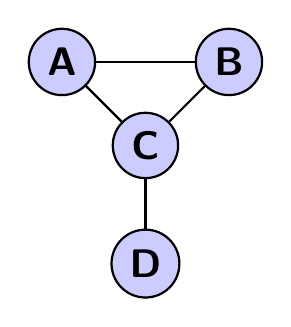
\begin{tikzpicture}[auto,node distance=1.5cm,
      thick,main node/.style={circle,fill=blue!20,draw,font=\sffamily\Large\bfseries}]


      \node[main node] (3) {C};
      \node[main node] (1) [above left of=3] {A};
      \node[main node] (2) [above right of=3] {B};
      \node[main node] (4) [below of=3] {D};


      \path[every node/.style={font=\sffamily\small}]
        (1) edge node {} (3)
            edge node {} (2)
        (2) edge node {} (3)
        (3) edge node {} (4);
    \end{tikzpicture}
  \end{center}

  \question[7] На графиката отгоре са изобразени четири маршрутизатора, които са
  конфигурирани за динамична маршрутизация с RIP. Ако не са имплементирани
  оптимизации за алгоритъма на Белман-Форд, какво ще бъде разстоянието между A и
  D след една стъпка от схождането на мрежата. (Приемете, че маршрутизаторите са
  били изключени до този момент)

  \begin{oneparchoices}
    \choice 1
    \CorrectChoice безкрайност
    \choice 3
    \choice 2
  \end{oneparchoices}

  \question[2] Кое от следните не е правилно разделяне на мрежата
  \texttt{10.0.0.0/22} на три подмрежи?

  \begin{choices}
    \choice \texttt{10.0.0.0/24}, \texttt{10.0.1.0/24}, \texttt{10.0.2.0/23}
    \CorrectChoice \texttt{10.0.0.0/23}, \texttt{10.0.2.0/24}, \texttt{10.0.3.0/24}
    \choice \texttt{10.0.0.0/24}, \texttt{10.0.1.0/23}, \texttt{10.0.3.0/24}
  \end{choices}

  \question[6] На кой слой от OSI модела работят маршрутизаторите?
  \begin{oneparchoices}
    \choice 1
    \choice 2
    \CorrectChoice 3
    \choice 4
    \choice 5
  \end{oneparchoices}

  \question[6] На кой слой от OSI модела работят комутаторите
  (\foreignlanguage{english}{switches})

  \begin{oneparchoices}
    \choice 1
    \CorrectChoice 2
    \choice 3
    \choice 4
    \choice 5
  \end{oneparchoices}

  \question[6] Маршрутната таблица съдържа: (изберете един верен отговор)
  \begin{choices}
    \choice съответствия между IP и MAC адреси
    \choice списък с всички MAC адреси на системи, с които хостът е разменял
    рамки
    \CorrectChoice списък на пътищата към IP мрежите, с които хостът може да
    разменя IP пакети
    \choice списък на всички IP aдреси, с които хостът е разменял IP пакети
  \end{choices}

  \question[6] RIP и OSPF са протоколи за:
  \begin{choices}
    \choice 
  \end{choices}

6. RIP (i OSPF) e protokol za
a) namirane na suotvetstvieto m/u IP address i MAC address
b) diagnostika na mrezhovi problemi
c) komunikacija m/u avtonomni sistemi (AS)
d) dinamichna razmjana na routes

7. BGP e
a) protokol, izpolzvan za komunikacija s naj-blizkija switch v lokalnata mrezha
b) IGP protokol
c) protokol za dinamichen routing, osnovno izpolzvan ot border routerite na avtonomnite sistemi
d) naslednik na TCP protokola

8. za TCP mozhem da kazhaem, che
a) ne garantira reliable data transmission
b) e protokol ot L3
c) garantira reliable data transmission
d) zadulzhitelno predava i IP adresite na komunikirashtite hostove, zashtoto IP protokola e unreliable

9. UDP dobavja pole za port s dulzhina
a) 8bit
b) 9bit
c) 12bit
d) 16bit
e) 18bit

10. porta, dobavjan ot TCP i UDP protokolite,
a) suvpada s poslednite 2 okteta ot mrezhovata maska
b) se maskira sus starshite 3 okteta na MAC adresa
c) adresira mrezhovite prilozhenija, kojto sa startirani na hosta
d) se polzva za namirane na default router-a

11. broja na validnite TCP/UDP portovete e
a) 255
b) 256
c) 32768
d) 65535
f) 262144
g) 4096

12. 10.0.0.0/28 mozhe da se razdeli na naj-mnogo
a) 2 podmrezhi
b) 3 podmrezhi
c) 4 podmrezhi
d) na mozhe da se razdeli na podmrezhi

13. 10.0.0.0/24 sudurzha podmrezhite
a) 10.0.1.0/25
b) 10.0.0.0/23
c) 10.0.1.0/24
d) 10.0.0.0/25
e) 10.0.2.0/25

14. komandata "echo 1 > /proc/sys/net/ipv4/ip_forward" pod Linux
a) aktivira routing podsistemata
b) spira aktivnija ethernet interface
c) uvelichava s 1 poslednija oktet ot adresa na hosta
d) zabranjava IPv6 protokola

15. ako sme v mrezha 10.0.0.0/24 i znaem, che imame router s adres 10.0.0.1 v mrezhata, s koja komanda dobavjame route kum mrezha 192.168.0.0/24
a) route add -net 192.168.0.0/24 gw 10.0.0.0
b) route add -net 192.168.0.0/24 gw 10.0.0.1
c) route add -net 192.168.0.0/24 gw 10.255.255.255
d) route add -net 192.168.0.0/24 gw 10.0.0.255
e) route add -net 192.168.255.255/24 gw 10.0.0.1

16. koja ot slednite mrezhi ne e validna v internet
a) 1.0.0.0/22
b) 2.0.0.0/24
c) 172.16.3.0/24
d) 200.0.0.0/22
e) 192.169.0.0/16

\end{questions}

%%% Local Variables: 
%%% mode: latex
%%% TeX-master: "test"
%%% TeX-PDF-mode: t
%%% End: 
